Ein weiteres weit verbreitetes Konzept sind Roboterfahrzeuge mit Reifen- oder
Rollenantrieb. Diese werden hauptsächlich bei niedrig wachsenden Sorten zur
Erkennung von Schädlingen oder beschädigten Pflanzen genutzt. Dies geschieht
durch hochauflösende Kamerasysteme und der Verarbeitung der Ergebnisse, zum
Teil mithilfe von künstlicher Intelligenz.

\begin{figure}[h]
	\centering
	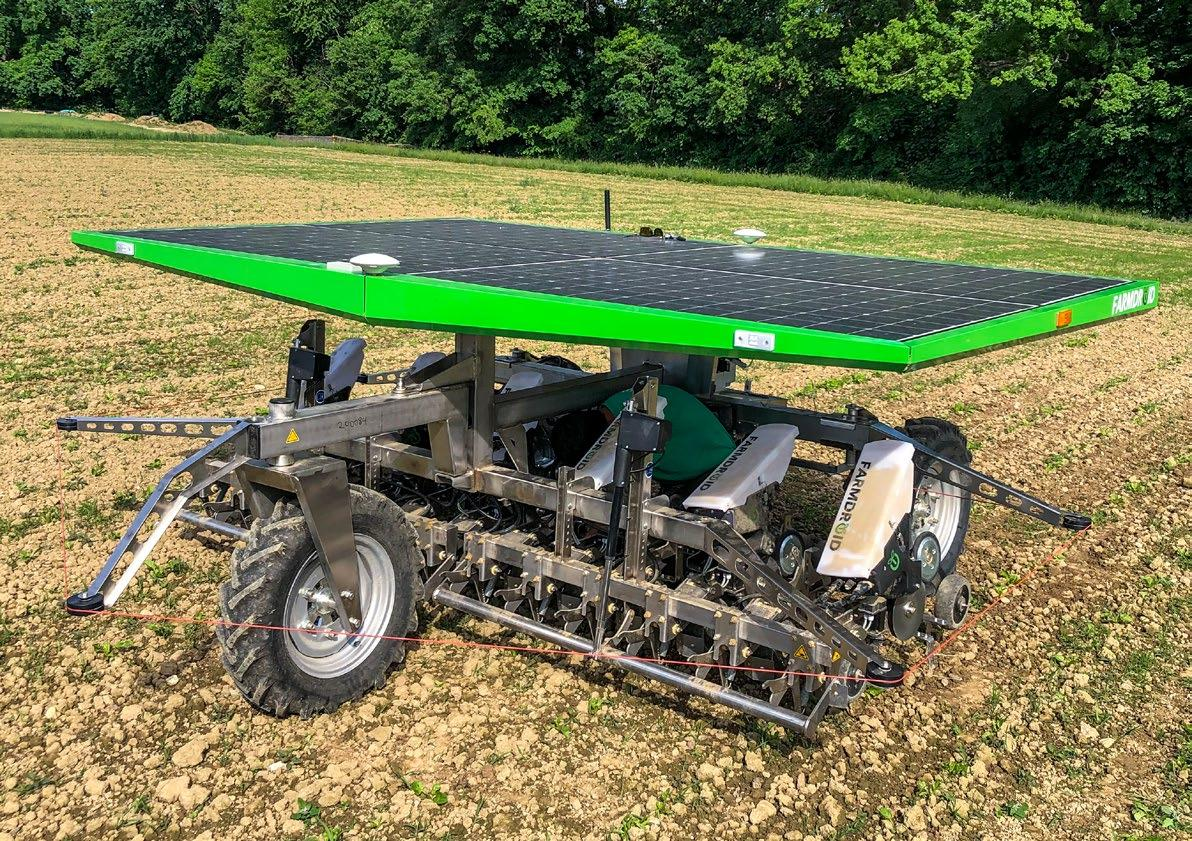
\includegraphics[width=0.7\textwidth]{bilder/farmdroid_fd20.png}
	\caption[Farmdroid FD20]{Farmdroid FD20}
	\label{fig:farmdroid_fd20}
\end{figure}

Der Farmdroid FD20 arbeitet hierbei komplett autonom und klimaneutral durch
Solarpanels. Diese Solarpanels können bei guter Sonneneinstrahlung mehr als
genug Energie für den Roboter liefern. Durch zwei zusätzliche Lithium-Ionen
Akkus ist es möglich, dass der Farmdroid auch nach Sonnenuntergang autark
weiterarbeitet, was einen Dauerbetrieb ermöglicht und damit extrem effizient
ist.\cite{jungwirth2022arbeitszeitbedarf}\\ Die Aufgabe des modernsten
Agrarroboters der Welt\cite{donaukurier2022} ist die Saat und die
Unkrautvernichtung. Laut Hersteller hat sich der Farmdroid bereits nach bis zu
1,5 Jahren amortisiert und arbeitet ab diesem Zeitpunkt aufgrund der
Solarpanels mit extrem niedrigen Unterhaltskosten. Zudem ist der Roboter
aufgrund der zwei GNSS Empfänger und eines RTK Korrektursignals, welches in der
Basisstation erzeugt wird, sehr genau.\cite{jungwirth2022arbeitszeitbedarf}